\documentclass[11pt]{beamer}
\usepackage{subcaption}
\usepackage{animate}
%Information to be included in the title page:
\title{Kimera: an Open-Source Library for Real-Time
Metric-Semantic Localization and Mapping}
\author{Ken Schlesiger}
\institute{Universität Würzburg}
\date{25.01.2024}
\definecolor{arsenic}{rgb}{0.0666, 0.0666, 0.10588}
\definecolor{text}{rgb}{0.8039, 0.8392, 0.95686}
\definecolor{headlines}{HTML}{89b4fa}
\definecolor{flamingo}{HTML}{f0c6c6}
\definecolor{pink}{HTML}{f5bde6}
\pagecolor{arsenic}
\setbeamercolor{background canvas}{bg=arsenic}
\setbeamercolor{normal text}{fg=text}
\setbeamercolor{frametitle}{fg=headlines}
\setbeamercolor{titlecolor}{fg=headlines}
\setbeamercolor{title}{fg=pink}
\setbeamercolor{caption name}{fg=pink}
\color{text}
% Define the information for the footline

% Customize the footline
\begin{document}
\addtobeamertemplate{title page}{}{
  \begin{beamercolorbox}[sep=1em,wd=\paperwidth,leftskip=0.5cm,rightskip=0.5cm]{footlinecolor}
  \end{beamercolorbox}
}

\frame[plain]{\titlepage}

\begin{frame}
\frametitle{}
\end{frame}
\begin{frame}
\frametitle{What does Kimera do?}
Three main Functions: 
\begin{itemize}
    \item Pose estimation (VIO) 
    \item 3D mesh reconstruction
    \item semantic mesh annotation
\end{itemize}
\end{frame}
\begin{frame}
\frametitle{The structure of Kimera}
Kimera is split into four parts:
\begin{itemize}
    \item Kimera-VIO
    \item Kiemra-RPGO
    \item Kimera-Mesher
    \item Kimera-Semantics
\end{itemize}
\end{frame}
\begin{frame}
\frametitle{The structure of Kimera}
\begin{figure}
    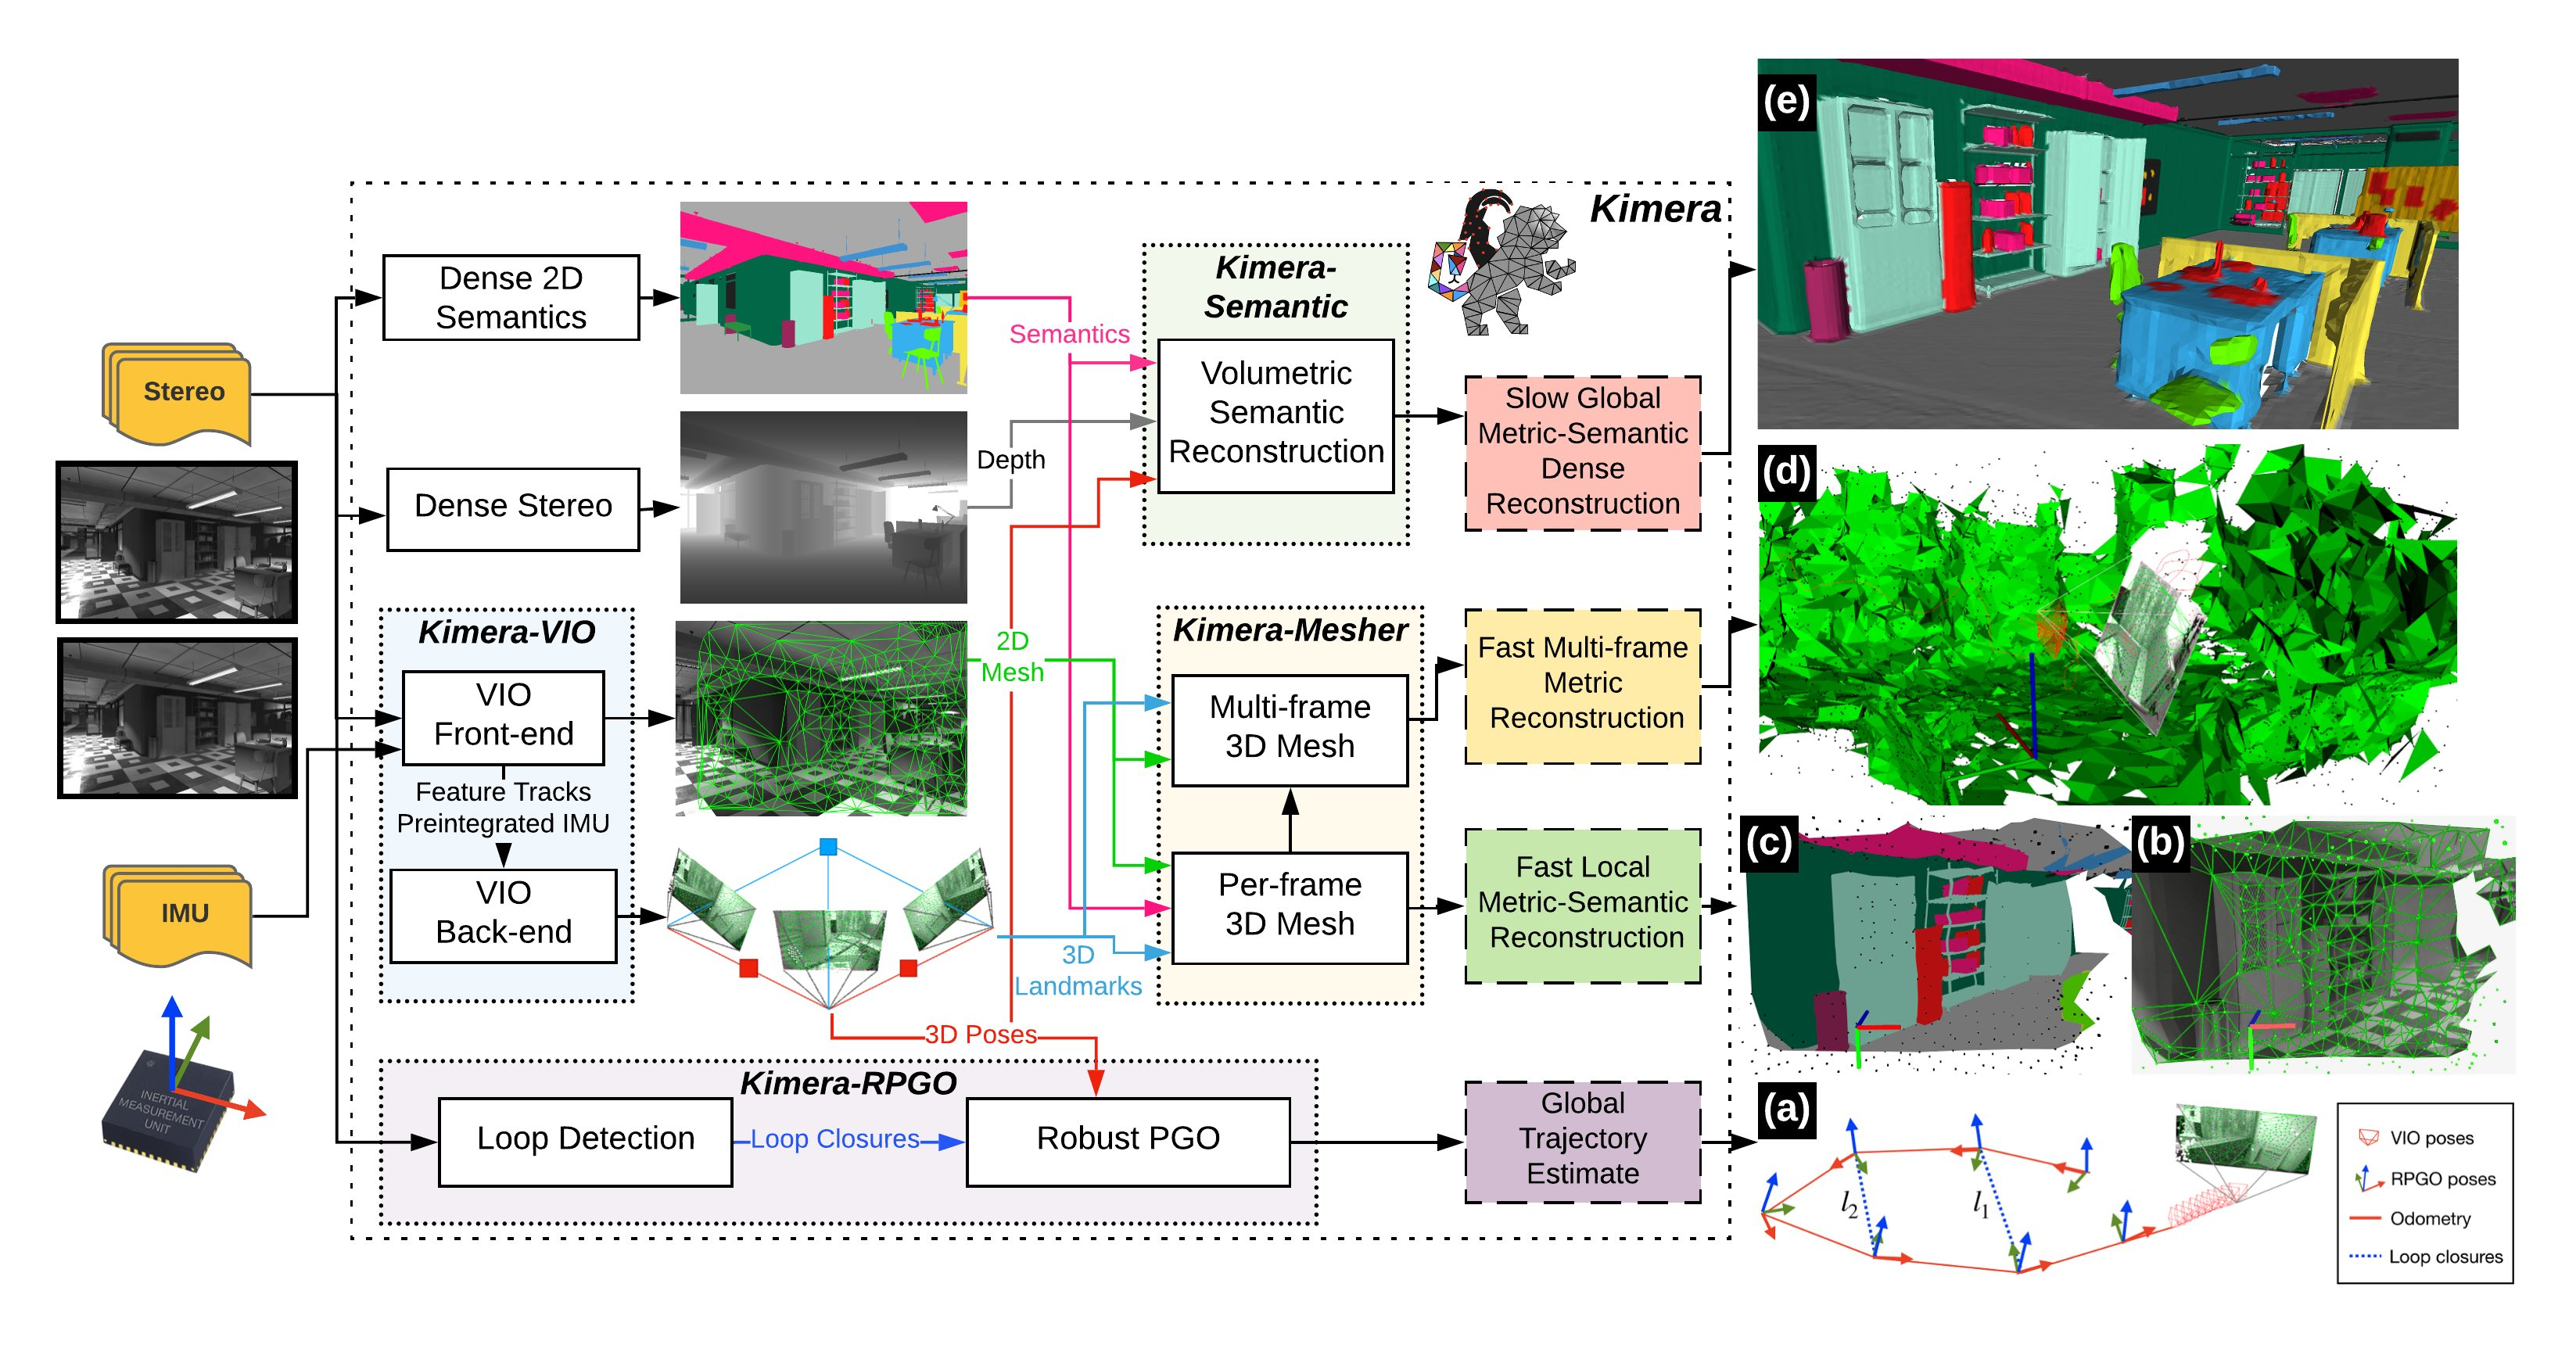
\includegraphics[width=\linewidth]{kimera_chart_23.jpeg} 
\end{figure}
\end{frame}
\begin{frame}
\frametitle{Kiera-VIO}
\begin{figure}
    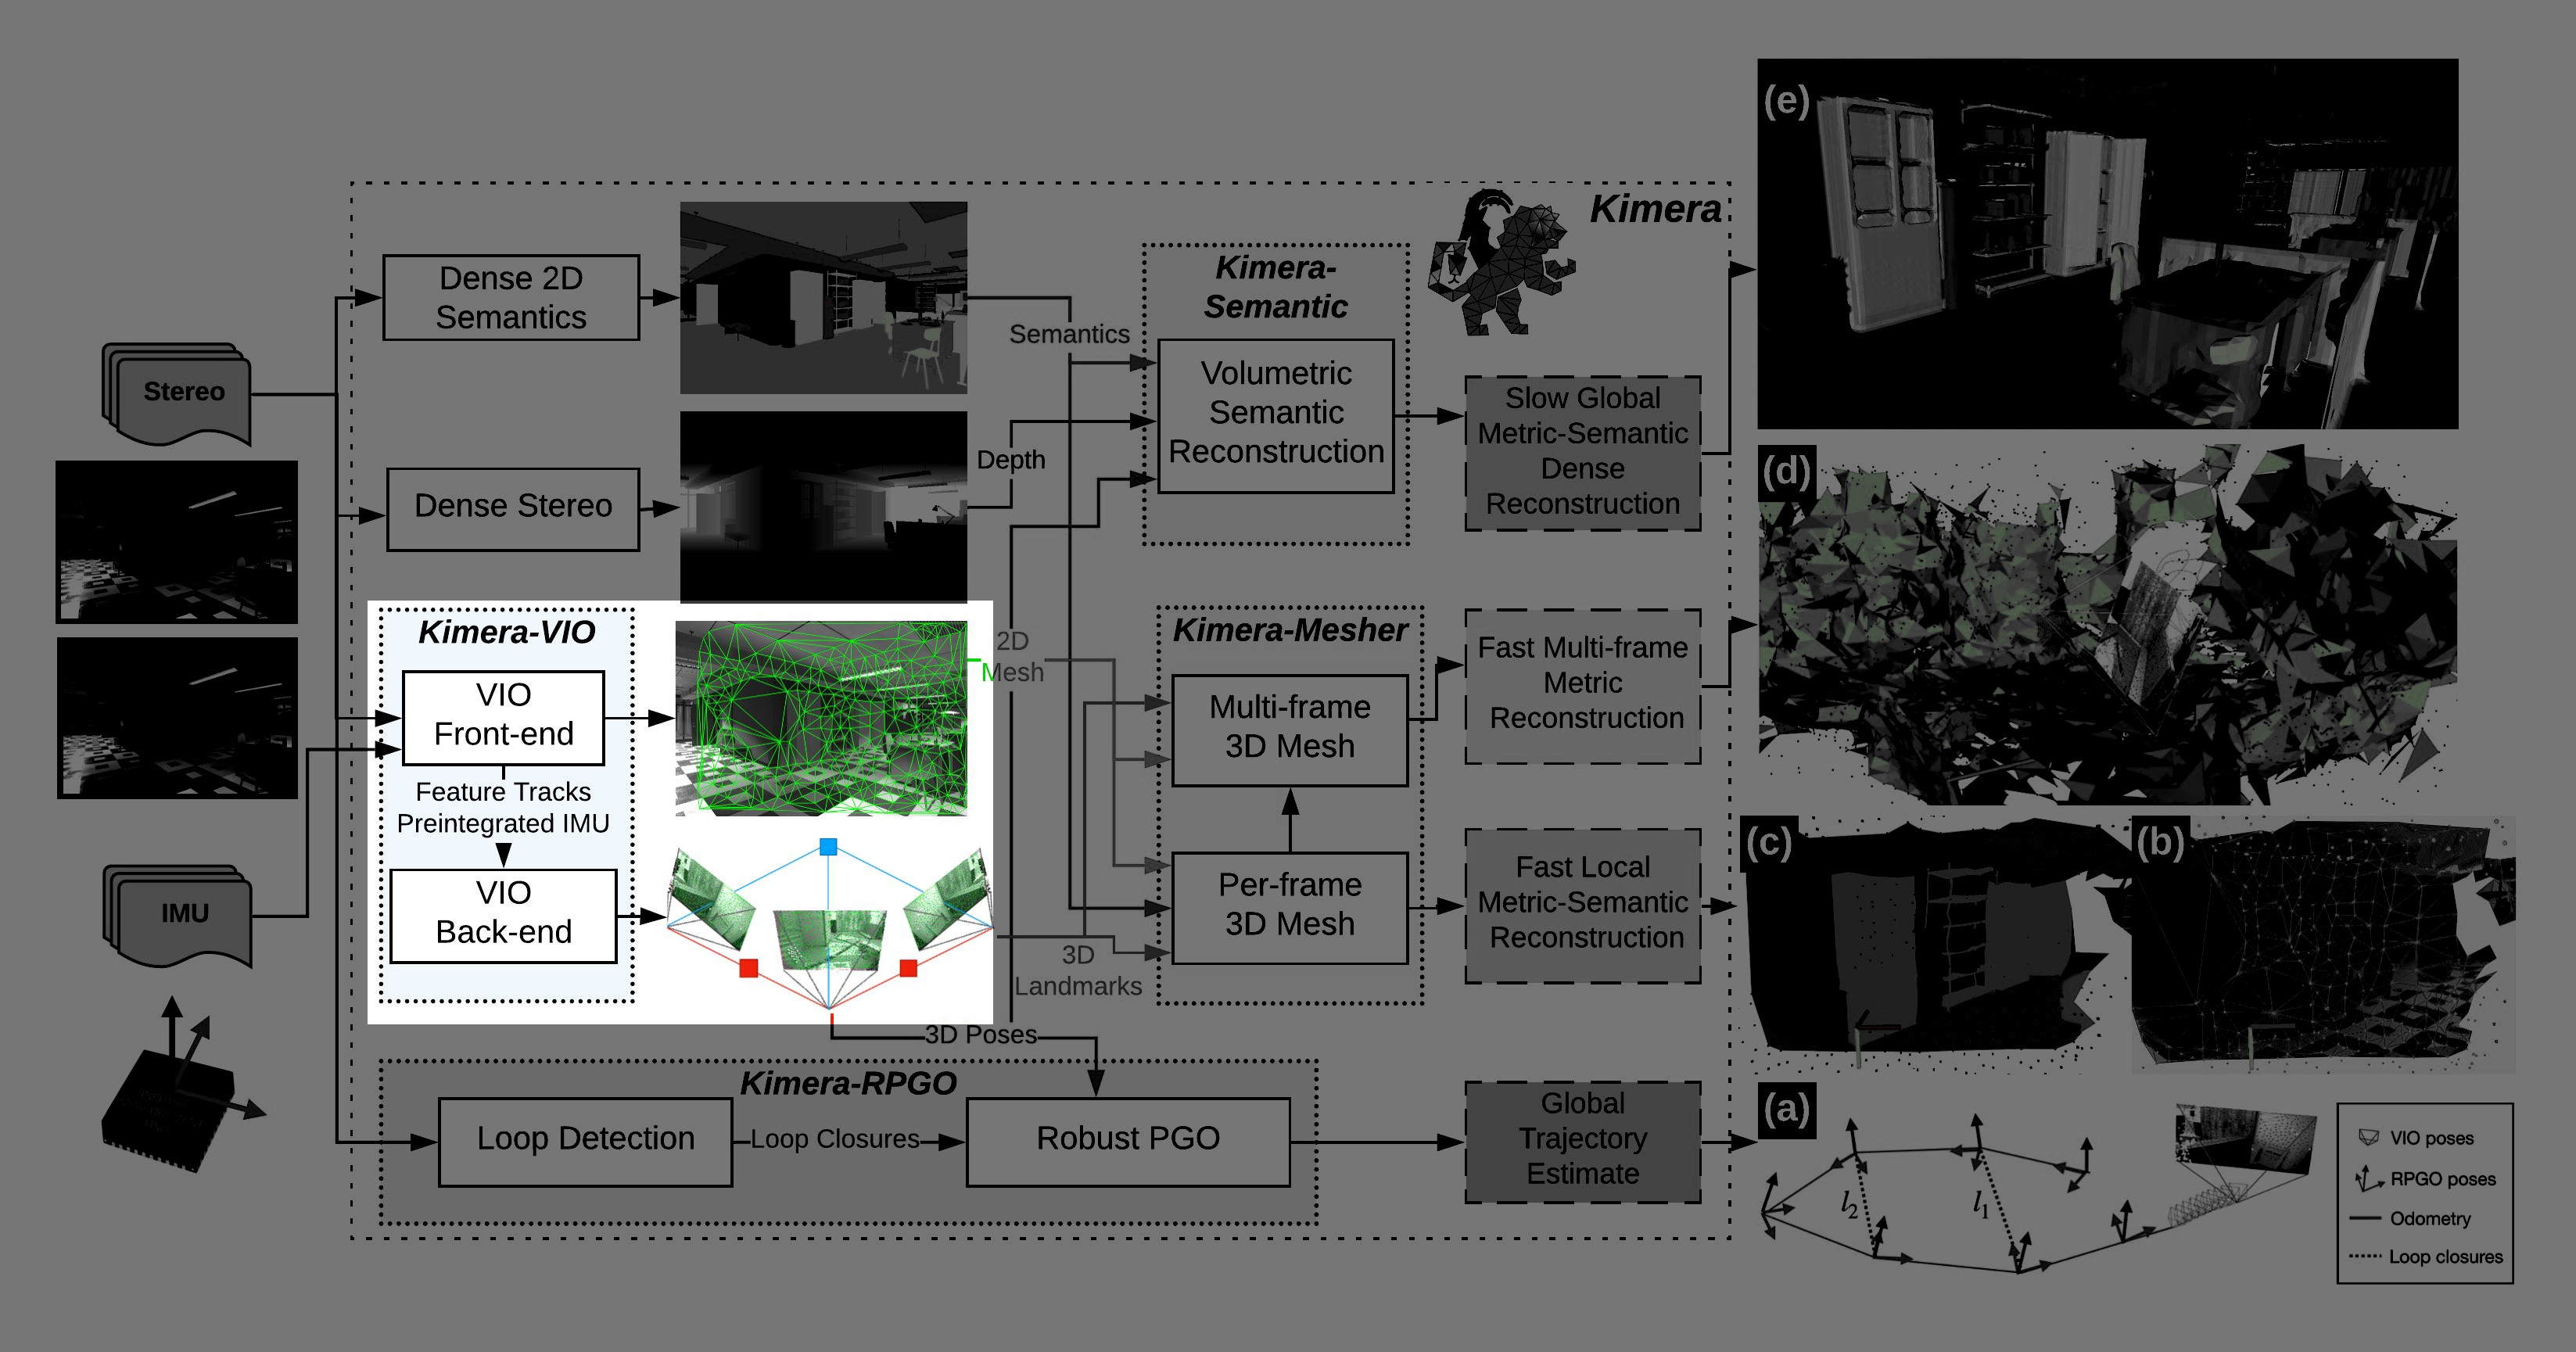
\includegraphics[width=\linewidth]{kimera_chart_VIO.jpeg} 
\end{figure}
\end{frame}
\begin{frame}
    \frametitle{Kimera-VIO} 
    \begin{figure}[ht]
        \centering
        \animategraphics[width=\linewidth,autoplay,loop]{12}{kimera_VIO_gif/kimeravio_ROS_mesh-}{0}{256}
    \end{figure}
\end{frame}
\begin{frame}[allowframebreaks]
\footnotesize
  \frametitle{References}
  \bibliographystyle{plain}
\bibliography{paper}{}
\end{frame}

\end{document}
